\chapter{Preliminaries}\label{preliminaries}
To get a better understanding of our research, we provide some preliminary information in this section. We will start by introducing the concept of \emph{reinforcement learning} in section \ref{pl-rl}. Following this, we will discuss \emph{state-space dimensionality reduction}, including several methods to do this in section \ref{pl-dimensionality}.
 
\section{Reinforcement learning}\label{pl-rl}
The main theoretical framework we are working in, is called \emph{reinforcement learning} (RL). This is a form of \emph{machine learning}, the area of artificial intelligence that is concerned with creating computer programs that can solve problems by learning from data. The two other main forms of machine learning are \emph{supervised learning} and \emph{unsupervised  learning}. The distinct feature of RL is that it learns from feedback through trial and error \cite[p. 2-5]{grokking}.

We will now examine RL more closely and formally, as well as discuss \emph{neural networks} and a specific RL algorithm used in our research called \emph{DQN}.

 
\subsection{General overview}
As mentioned, RL is the area of artificial intelligence where problems are solved through trial and error using feedback. An example is a robot learning to bring a given package to a given location. The portion of the code responsible for the decision making, i.e. choosing an action, is called the \emph{agent}. Besides an agent, there is also the \emph{environment}, which entails everything other than the agent. In our package delivery example this could for instance be the hardware of the robot, the package to be delivered, wind conditions, the road, and any obstacle.

The environment is encoded in a set of variables, where all possible values of these variables are called the \emph{state-space}. In our example, some of these variables are the coordinates of the location of the robot, wind speed and direction, and the coordinates for the location where the package needs to be delivered. A single instantiation of the state-space is a \emph{state}. 

To be able to make any informed decision, the agent will need some information with regards to the current state. The information about a state received by the agent, i.e. the variables making up the state-space, is called an \emph{observation}. This observation might be partial; the agent might not receive all information about a state. In our example, the agent might not have any information about an obstacle on the road that it hasn't sensed yet.

Using this information, the agent makes a decision  about which action to take. A lot of different algorithms exist with regards to decision making and learning how to make better decision. In section \ref{pl-dqn} we will discuss the learning algorithm we will use, called \emph{deep-Q-network}. Depending on the current state and the action taken by the agent, the environment might go to a new, different state. This change is encoded by a \emph{transition function}; given a state and action pair it returns the next state. 

The current mapping in the agent between a given state and a chosen action is called its \emph{policy}. The better its policy, the better it is able to solve the problem. To be able to improve its policy, the agent needs information about how well it has been performing. This feedback is given in the form of \emph{rewards}: the environment sends positive or negative rewards to the agent, informing it about how well it has performed. In our package delivery example, the robot might get a $+1$ reward whenever it delivers a package.

This results in an interaction cycle between the agent and the environment, depicted in figure \ref{fig:rl_cycle}. It begins with the agent receiving an observation. Then, it chooses an action. This results in the environment transitioning into a new state (possibly the same state as before having taken the action). After this, the environment send a new observation along with a reward to the agent, and the the agent chooses a new action. This interaction stops once the problem has been solved, or when some other constraint has been violated (like a time limit, or the robot getting into an unwanted state like the robot crashing into an object). When the cycle stops, we have finished an \emph{episode}. After this, the environment can be reset to start a new episode. To get to a well performing policy, the agent often needs hundreds or thousands of episodes \cite[p. 6-10]{grokking}. 

\begin{figure}[h]
    \centering
    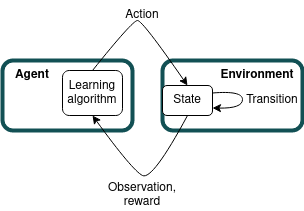
\includegraphics[width=0.75\textwidth]{rl-cycle}
    \caption{The cycle of interaction between the environment and an agent in reinforcement learning.}
    \label{fig:rl_cycle}
\end{figure}

Let us now formally define the reinforcement learning paradigm. 

\subsection{Neural networks}
deep rl (grokking p 5)
neural networks (incl non-linnear function approximation)
\subsection{(D)DQN}\label{pl-dqn}
si 

\section{State-space dimensionality reduction}\label{pl-dimensionality}
Definition, general info
Methods:
\subsection{Principal Component Analysis}\label{pl-pca}
algemene info pca
\subsection{Autoencoder}\label{pl-ae}
Another way of projecting data onto a lower dimensional space, is using an \emph{autoencoder}\cite{AE_general}. An autoencoder is a neural network consisting of two parts: an encoder network and a decoder network. The encoder projects the given input data onto a lower dimensional space, also called the \emph{latent space}. The output of the encoder, called the \emph{latent representation}, is used as input for the decoder. This decoder tries to reconstruct the original input from the latent representation as closely as possible. The autoencoder architecture is shown in figure \ref{fig:AE_architecture}.

\begin{figure}[h]
    \centering
    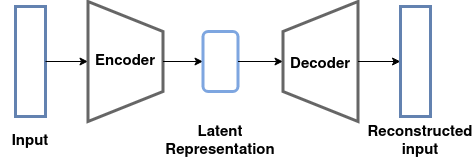
\includegraphics[width=0.75\textwidth]{AE_architecture}
    \caption{The architecture of an autoencoder.}
    \label{fig:AE_architecture}
\end{figure}

Formally, an autoencoder can be defined by the two functions it learns: 
\begin{equation}
  \label{enc}
  \phi :{\mathbb{R}^n}\rightarrow {\mathbb{R}^m}
\end{equation}
\begin{equation}
  \label{dec}
  \psi :{\mathbb{R}^m}\rightarrow {\mathbb{R}^n}
\end{equation}
\begin{equation}
  \label{encdec}
  \phi ,\psi ={\underset {\phi ,\psi }{\operatorname {arg\,min} }}\,{\Delta}(x, \psi \circ \phi (x))
\end{equation}
Equation~\eqref{enc} defines the encoder and equation~\eqref{dec} the decoder, both satisfying~\eqref{encdec} where $\Delta$ is the reconstruction loss function for input x. The closer the output of the autoencoder approximates the original input, the lower the loss.

A fundamental difference with using PCA, is the type of functions that can be approximated for lowering the dimensionality. Since an autoencoder uses neural networks, they can approximate nonlinear functions, as mentioned in section \ref{pl-rl}. This is in contrast with PCA, which can only approximate linear functions. Because of this, an autoencoder can learn more powerful generalisations which leads to lower information loss\cite{AE_general}.

\subsection{DeepMDP}\label{pl-deepmdp}
Info over deepmdp
